\documentclass{article}
\usepackage{JASA_manu} %formats document like ASA wants
\usepackage{jasa_harvard} %formats citations like ASA wants
\usepackage{amssymb, amsmath, amsthm, graphics, graphicx, color, fullpage}
\usepackage{thmtools} %to format the Algorithm environment correctly
\usepackage{nameref, hyperref, cleveref} %for named references
\usepackage{zref-xr, zref-user} %for hyperlinked references to outside docs

% define algorithm environment
\declaretheoremstyle[
notefont=\bfseries, notebraces={}{},
bodyfont=\normalfont\itshape,
headformat=\NAME:\NOTE
]{nopar}
\declaretheorem[style=nopar, name=Algorithm, 
refname={Algorithm,Algorithms},
Refname={Algorithm,Algoritms},
numbered=no]{alg*}

\newtheorem{thm}{Theorem}[subsection]
\newtheorem{prop}[thm]{Proposition}
\newtheorem{cor}[thm]{Corollary}
\newtheorem{lem}[thm]{Lemma}

\DeclareMathOperator{\tr}{tr}
\DeclareMathOperator{\B}{B}
\DeclareMathOperator{\vech}{vech}
\DeclareMathOperator{\vect}{vec}

\graphicspath{{plots/}}
\newcommand{\matt}[1]{{\color{red} Matt: #1}}
\newcommand{\jarad}[1]{{\color{red} Jarad: #1}}


\begin{document}


\title{Appendices for Interweaving Markov chain Monte Carlo strategies for efficient
estimation of dynamic linear models}
\author{Matt Simpson, Jarad Niemi, Vivekananda Roy}
\maketitle
\appendix
\section{Full conditional distributions in the general DLM for various DAs}\label{sec:DLMfullcond}

The class of DLMs we consider is defined as follows:
\begin{align}
y_t &= F_t\theta_t + v_t && v_t \stackrel{ind}{\sim} N_k(0,V) && (\mbox{observation equation}) \label{dlmtdobseq}\\
 \theta_t &= G_t\theta_{t-1} + w_t && w_t \stackrel{ind}{\sim} N_p(0,W) && (\mbox{system equation}) \label{dlmtdsyseq}
\end{align}
for $t=1,2,\cdots T$ with the priors $\theta_0 \sim N_p(m_0, C_0)$, $V \sim IW(\Lambda_V, \lambda_V)$ and $W \sim IW(\Lambda_W, \lambda_W)$ with $(\theta_0,V,W)$ mutually independent. Then the full joint distribution of $(V,W,\theta,y)$ is
\begin{align}
  p(&V,W,\theta,y) \propto \exp\left[-\frac{1}{2}(\theta_0-m_0)'C_0^{-1}(\theta_0-m_0)\right] \nonumber\\
  &\times   |V|^{-(\lambda_V + k + T + 2)/2}\exp\left[-\frac{1}{2}\tr\left(\Lambda_VV^{-1}\right)\right] \exp\left[-\frac{1}{2}\sum_{t=1}^T(y_t - F_t\theta_t)'V^{-1}(y_t - F_t\theta_t)\right] \nonumber\\
   & \times |W|^{-(\lambda_W + p + T + 2)/2}\exp\left[-\frac{1}{2}\tr\left(\Lambda_WW^{-1}\right)\right]\exp\left[-\frac{1}{2}\sum_{t=1}^T(\theta_t-G_t\theta_{t-1})'W^{-1}(\theta_t-G_t\theta_{t-1})\right]\label{dlmjoint}
 \end{align}
where $\tr(.)$ is the matrix trace operator.

In the following subsections, we provide derivations of the full conditional distributions for when using states, scaled disturbances or scaled errors as the data augmentation. 

\subsection{States}\label{subsec:states}

With the usual DA, the full conditional distributions can be derived from equation \eqref{dlmjoint}. First, the full conditional distribution of $\theta$ is as follows:
\begin{align*}
p(\theta&|V,W,y) \propto p(V,W,\theta,y) \propto \exp\left[-\frac{1}{2}(\theta_0-m_0)'C_0^{-1}(\theta_0-m_0)\right] \\
  &\times \exp\left[-\frac{1}{2}\sum_{t=1}^T(y_t - F_t\theta_t)'V^{-1}(y_t - F_t\theta_t)\right] \exp\left[-\frac{1}{2}\sum_{t=1}^T(\theta_t-G_t\theta_{t-1})'W^{-1}(\theta_t-G_t\theta_{t-1})\right].
\end{align*}
It turns out that this density is Gaussian. In Section \ref{sec:MCFA}, we show how to use the mixed Cholesky factorization algorithm (MCFA) in order to efficiently determine and draw from this distribution.

The full conditional of $(V,W)$ is:
\begin{align*}
  p(V,W&|\theta,y) \propto p(V,W,\theta,y) \propto  |V|^{-(\lambda_V + k + T + 2)/2}\exp\left[-\frac{1}{2}\tr\left(\Lambda_VV^{-1}\right)\right] \exp\left[-\frac{1}{2}\sum_{t=1}^T(y_t - F_t\theta_t)'V^{-1}(y_t - F_t\theta_t)\right]\\
   & \times |W|^{-(\lambda_W + p + T + 2)/2}\exp\left[-\frac{1}{2}\tr\left(\Lambda_WW^{-1}\right)\right]\exp\left[-\frac{1}{2}\sum_{t=1}^T(\theta_t-G_t\theta_{t-1})'W^{-1}(\theta_t-G_t\theta_{t-1})\right]\\
&\propto |V|^{-(\lambda_V + k + T + 2)/2}\exp\left[-\frac{1}{2}\tr\left(\left(\Lambda_V +  \sum_{t=1}^T(y_t - F_t\theta_t)(y_t - F_t\theta_t)'\right) V^{-1}\right)\right]\\
 &\times |W|^{-(\lambda_W + p + T + 2)/2}\exp\left[-\frac{1}{2}\tr\left(\left(\Lambda_W  + \sum_{t=1}^T(\theta_t-G_t\theta_{t-1})(\theta_t-G_t\theta_{t-1})'\right)W^{-1}\right)\right].
 \end{align*}
In other words, $V$ and $W$ are conditionally independent given $y$ and $\theta$ with
\begin{align*}
  V|\theta,y &\sim IW\left(\Lambda_V + \sum_{t=1}^Tv_tv_t',\lambda_V + T\right), &
  W|\theta,y &\sim IW\left(\Lambda_W + \sum_{t=1}^Tw_tw_t',\lambda_{W} + T\right) 
\end{align*}
where $v_t = y_t - F_t\theta_t$ and $w_t = \theta_t - G_t\theta_{t-1}$.

\subsection{Scaled disturbances}\label{subsec:SDs}

Let $L_W$ denote the Cholesky decomposition of $W$, i.e. the lower triangle matrix $L_W$ such that $L_WL_W' =W$. Then the scaled disturbances are $\gamma=\gamma_{0:T}=(\gamma_0',\gamma_1',\cdots,\gamma_T')'$ defined by $\gamma_0=\theta_0$ and $\gamma_t = L_W^{-1}(\theta_t-G_t\theta_{t-1})$ for $t=1,2,\cdots,T$. The reverse transformation is defined recursively by $\theta_0=\gamma_0$ and $\theta_t=L_W\gamma_t + G_t\theta_{t-1}$ for $t=1,2,\cdots,T$. Then the Jacobian is block lower triangular with the identity matrix and $T$ copies of $L_W$ along the diagonal blocks, so $|J| = |L_W|^T=|W|^{T/2}$. From equation \eqref{dlmjoint} we can write the full joint distribution of $(V,W,\gamma,y)$ as
 \begin{align}
  p(&V,W,\gamma,y) \propto \exp\left[-\frac{1}{2}(\gamma_0-m_0)'C_0^{-1}(\gamma_0-m_0)\right] \exp\left[-\frac{1}{2}\gamma_t'\gamma_t\right] \nonumber\\
  &\times |W|^{-(\lambda_W + p + 2)/2} |V|^{-(\lambda_V + k + T + 2)/2} \exp\left[-\frac{1}{2}\tr\left(\Lambda_WW^{-1}\right)\right]  \nonumber\\
  &\times \exp\left[-\frac{1}{2}\left(\tr\left(\Lambda_VV^{-1}\right) + \sum_{t=1}^T\left[y_t-F_t\theta_t(\gamma,W)\right]'V^{-1}\left[y_t-F_t\theta_t(\gamma,W)\right]\right)\right]\label{dlmdistjoint}. 
 \end{align}
where $\theta_t(\gamma,W)$ denotes the recursive back transformation defined by the scaled disturbances. The full conditional distribution of $\gamma$ is then
\begin{align*}
  p(\gamma&|V,W,y) \propto p(V,W,\gamma,y) \propto \exp\left[-\frac{1}{2}(\gamma_0-m_0)'C_0^{-1}(\gamma_0-m_0)\right] \exp\left[-\frac{1}{2}\gamma_t'\gamma_t\right]\\
&\times \exp\left[-\frac{1}{2}\left(\sum_{t=1}^T\left[y_t-F_t\theta_t(\gamma,W)\right]'V^{-1}\left[y_t-F_t\theta_t(\gamma,W)\right]\right)\right]. 
\end{align*}
This density is Gaussian, but difficult to draw from. We use the MCFA to draw from $\theta|V,W,y$ instead, then transform from $\theta$ to $\gamma$ using the definition of $\gamma$.

Under this parameterization, the full conditional distribution of $(V,W)$ is
 \begin{align*}
  p(&V,W,|\gamma,y) \propto  p(V,W,\gamma,y) |W|^{-(\lambda_W + p + 2)/2} |V|^{-(\lambda_V + k + T + 2)/2} \exp\left[-\frac{1}{2}\tr\left(\Lambda_WW^{-1}\right)\right]  \nonumber\\
  &\times \exp\left[-\frac{1}{2}\left(\tr\left(\Lambda_VV^{-1}\right) + \sum_{t=1}^T\left[y_t-F_t\theta_t(\gamma,W)\right]'V^{-1}\left[y_t-F_t\theta_t(\gamma,W)\right]\right)\right]. 
 \end{align*}
The back transformation from $\theta$ to $\gamma$ sets $\theta_0=\gamma_0$ and for $t=1,2,\cdots,T$
\begin{align*}
\theta_t &= L_W\gamma_t + G_t\theta_{t-1}\\
&= L_W\gamma_t + \sum_{s=0}^{t-2}G_tG_{t-1}\hdots G_{t-s}L_W\gamma_{t-s-1} + G_tG_{t-1}\hdots G_1\gamma_0\\
&= \sum_{s=0}^{t-1}\tilde{G}_{s,t}L_W\gamma_{t-s} + \tilde{G}_{t,t}\gamma_0
\end{align*}
where $\tilde{G}_{s,t} = G_tG_{t-1}\cdots G_{t-s + 1}$ for $s >0$ and $\tilde{G}_{0,t}=I_p$, the $p\times p$ identity matrix.. Then we can rewrite the conditional distribution of $(V,W)$ as
 \begin{align*}
  p(&V,W,|\gamma,y) \propto  p(V,W,\gamma,y) \propto |W|^{-(\lambda_W + p + 2)/2} |V|^{-(\lambda_V + k + T + 2)/2} \exp\left[-\frac{1}{2}\tr\left(\Lambda_WW^{-1}\right)\right] \exp\left[-\frac{1}{2}\left(\tr\left(\Lambda_VV^{-1}\right)\right)\right]  \nonumber\\
  &\times  \exp\left[-\frac{1}{2}\left(\sum_{t=1}^T\left[y_t-F_t\sum_{s=0}^{t}\tilde{G}_{s,t}L_W\gamma_{t-s} - F_t\tilde{G}_{t,t}\gamma_0\right]'V^{-1}\left[y_t-F_t\sum_{s=0}^{t-1}\tilde{G}_{s,t}L_W\gamma_{t-s} - F_t\tilde{G}_{t,t}\gamma_0\right]\right)\right]. 
 \end{align*}
This density is fairly complicated, so we resort to the full conditionals of $V$ and $W$ separately. The full conditional of $V$ is familiar:
 \begin{align*}
  p(&V|W,\gamma,y) \propto  p(V,W|\gamma,y) \propto |V|^{-(\lambda_V + k + T + 2)/2} \times \exp\left[-\frac{1}{2}\left(\tr
\left[\Lambda_V + \sum_{t=1}^Tv_tv_t'\right]V^{-1}\right)\right]
 \end{align*}
where $v_t = y_t - F_t\sum_{s=0}^{t}\tilde{G}_{s,t}L_W\gamma_{t-s} - F_t\tilde{G}_{t,t}\gamma_0 = y_t - F_t\theta_t$. This implies that
\begin{align*}
  V|W,\gamma,y &\sim IW\left(\Lambda_V + \sum_{t=1}^Tv_tv_t',\lambda_V + T\right)
\end{align*}
which is the same distribution as for $V|\theta,y$. 

The full conditional density of $W$ is more complicated:
 \begin{align*}
  p(W&|V,\gamma,y) \propto  p(V,W,\gamma,y) \propto |W|^{-(\lambda_W + p + 2)/2}\exp\left[-\frac{1}{2}\tr\left(\Lambda_WW^{-1}\right)\right]\\
&\times  \exp\left[-\frac{1}{2}\left(\sum_{t=1}^T\left[y_t-F_t\sum_{s=0}^{t}\tilde{G}_{s,t}L_W\gamma_{t-s} - F_t\tilde{G}_{t,t}\gamma_0\right]'V^{-1}\left[y_t-F_t\sum_{s=0}^{t-1}\tilde{G}_{s,t}L_W\gamma_{t-s} - F_t\tilde{G}_{t,t}\gamma_0\right]\right)\right]. 
 \end{align*}
In the local level model, the density is even simpler. The local level model assumes that $y_t$ and $\theta_t$ are univariate for all $t$ and that $F_t=G_t=1$. In addition, the prior on $W$ reduces to an inverse gamma prior, $IG(\alpha_W,\beta_W)$. In this case, the full conditional density of $W$ becomes
\begin{align*}
  p(W&|V,\gamma,y) \propto W^{-\alpha_W   - 1}\exp\left[-\frac{1}{W}\beta_W  \right]  \exp\left[-\frac{1}{2}\left(\sum_{t=1}^T\left[y_t-\sum_{s=0}^{t}\gamma_{t-s}\sqrt{W}\right]'V^{-1}\left[y_t-\sum_{s=0}^{t-1}\gamma_{t-s}\sqrt{W}\right]\right)\right]\\
&\propto W^{-\alpha_W - 1}\exp\left[-a_\gamma W + b_\gamma \sqrt{W} -\frac{\beta_W}{W}\right]. 
\end{align*}
where $a_\gamma =\sum_{t=1}^T(\sum_{s=1}^t\gamma_j)^2/2V$ and $b_\gamma =\sum_{t=1}^T(y_t-\gamma_0)(\sum_{s=1}^t\gamma_j)/V$. In Section \ref{sec:scaledraw} we show how to efficiently obtain a random draw from this density.

\subsection{Scaled errors}\label{subsec:SEs}
Let $L_V$ denote the Cholesky decomposition of $V$, that is $L_VL_V'=V$, then we can define the scaled errors as $\psi_t = L_V^{-1}(y_t - F_t\theta_t)$ for $t=1,2,\cdots,T$ and $\psi_0 = \theta_0$. Here we assume that $k=p$ and that $F_t$ is invertible for all $t$. Then the back transformation is $\theta_t = F_t^{-1}(y_t - L_V\psi_t)$ for $t=1,2,\cdots,T$ and $\theta_0=\psi_0$. The Jacobian of this transformation is block diagonal with a single copy of the identity matrix along with the $F_t^{-1}L_V$'s along the diagonal, so $|J|=(\prod_{t=1}^T|F_t|^{-1})|V|^{T/2}$. Then from equation \eqref{dlmjoint} we can write the joint distribution of $(V, W, \psi, y)$ as
\begin{align}
    p(&V,W,\psi,y) \propto \exp\left[-\frac{1}{2}(\psi_0-m_0)'C_0^{-1}(\psi_0-m_0)\right] \exp\left[-\frac{1}{2}\sum_{t=1}^T\psi_t'\psi_t\right] \nonumber\\
  &\times |V|^{-(\lambda_V + p + 2)/2}\exp\left[-\frac{1}{2}\tr\left(\Lambda_VV^{-1}\right)\right]  \times |W|^{-(\lambda_W + p + T + 2)/2} \nonumber\\
   & \exp\left[-\frac{1}{2}\left(\tr\left(\Lambda_WW^{-1}\right) + \sum_{t=1}^T(y_t - \mu_t)'(F_tWF_t')^{-1}(y_t-\mu_t)\right)\right]\label{dlmerrorjoint}
\end{align}
where we define $\mu_1 = L_V\psi_1 + F_1G_1\psi_0$ and for $t=2,3,\cdots,T$, $\mu_t =L_V\psi_t + F_tG_tF_{t-1}^{-1}(y_{t-1} - L_{V}\psi_{t-1})$. The $|F_t|^{-1}$'s have been absorbed into the normalizing constant, but if they depended on some unknown parameter then we could not do this and as a result would have to take them into account in the Gibbs step or steps for the model parameters.

The full conditional distribution of $\psi$ is
\begin{align*}
    p(&V,W,\psi,y) \propto \exp\left[-\frac{1}{2}(\psi_0-m_0)'C_0^{-1}(\psi_0-m_0)\right] \exp\left[-\frac{1}{2}\sum_{t=1}^T\psi_t'\psi_t\right] \nonumber\\
   & \exp\left[-\frac{1}{2}\left(\sum_{t=1}^T(y_t - \mu_t)'(F_tWF_t')^{-1}(y_t-\mu_t)\right)\right]
\end{align*}
where note that $\mu_t$ depends on $\psi$. This density is Gaussian and like with $\gamma$, we can use the MCFA from Section \ref{sec:MCFA} to draw from the full conditional of $\theta$ and then transform from $\theta$ to $\psi$. However it turns out the precision matrix of $\psi$'s full conditional distribution has the necessary block tridiagonal structure, so we use the MCFA directly on $\psi$. 

The full conditional distribution of $(V,W)$ is complicated, like the case of the scaled disturbances, so we find the full conditionals of $V$ and $W$ separately instead. The full conditional of $W$ is 
\begin{align*}
 p(&W|V,\psi,y) \propto   p(V,W,\psi,y) \propto \times |W|^{-(\lambda_W + p + T + 2)/2} \exp\left[-\frac{1}{2}\left(\tr\left(\left[\Lambda_W + \sum_{t=1}^TF_t^{-1}(y_t - \mu_t)(y_t-\mu_t)'(F_t^{-1})'\right]W^{-1}\right)\right)\right],
\end{align*}
in other words
\begin{align*}
  W|V,\psi,y &\sim IW\left(\Lambda_W + \sum_{t=1}^Tw_tw_t',\lambda_{W} + T\right) 
\end{align*}
where $w_t = F_t^{-1}(y_t - \mu_t) = \theta_t - G_t\theta_{t-1}$.

The full conditional distribution of $V$ is more complicated:
\begin{align*}
 p(V&|W,\psi,y) \propto p(V,W,\psi,y) \propto |V|^{-(\lambda_V + p + 2)/2}\exp\left[-\frac{1}{2}\tr\left(\Lambda_VV^{-1} + \sum_{t=1}^T(y_t - \mu_t)'(F_tWF_t')^{-1}(y_t-\mu_t)\right)\right]
\end{align*}
with $\mu_t$ a function of $V$, defined above. In the local level model with an $IG(\alpha_V,\beta_V)$ prior on $V$, this density is simpler:
\begin{align*}
 p(V&|W,\psi,y) \propto V^{-alpha_V - 1}\exp\left[-\frac{\beta_V}{V} + \frac{1}{W}\sum_{t=1}^T(y_t - \mu_t)'(y_t-\mu_t)\right]
\end{align*}
where $\mu_1 = \sqrt{V}\psi_1 + \psi_0$ and for $t=2,3,\cdots,T$, $\mu_t = \sqrt{V}(\psi_t - \psi_{t-1}) + y_{t-1}$. Thus
\begin{align*}
 p(V|W,\psi,y) \propto V^{-\alpha_V - 1}\exp\left[ -a_{\psi}V + b_{\psi}\sqrt{V} -\frac{\beta_V}{V}\right] 
\end{align*}
where $a_{\psi}=\sum_{t=1}^T(L\psi_t)^2/2W$ and $b_{\psi}=\sum_{t=1}^T(L\psi_tLy_t)/W$, and we define $Ly_t=y_t-y_{t-1}$ for $t=2,3,\cdots,T$, $Ly_1=y_1 - \psi_0$, $L\psi_t = \psi_t - \psi_{t-1}$ for $t=2,3,...,T$ and $L\psi_1=\psi_1-0$. In other words, the form of $p(V|W,\psi,y)$ is the same as $p(W|V,\gamma,y)$. The general form of these two densities is $p(x)\propto x^{-\alpha-1}\exp\left[ -ax + b\sqrt{x} -c/x\right]$. In Section \ref{sec:scaledraw} we show how to efficiently sample from this distribution.

\subsection{The wrongly-scaled disturbances}\label{subsec:WSDs}

The wrongly-scaled disturbances are defined as  $\tilde{\gamma}=\tilde{\gamma}_{0:T}=(\tilde{\gamma}_0',\tilde{\gamma}_1',\cdots,\tilde{\gamma}_T')'$. The wrongly-scaled disturbances are related to the scaled disturbances by $\tilde{\gamma}_t = L_V^{-1}L_W\gamma_t$ for $t=1,2,\cdots,T$ and $\tilde{\gamma_0}=\gamma_0$. The reverse transformation is $\gamma_t = L_W^{-1}L_V\tilde{\gamma}_t$ and the Jacobian is block diagonal with a copy of the identity matrix and $T$ copies of $L_W^{-1}L_V$ along the diagonal. Thus $|J|=|L_W|^{-T}|L_V|^T=|W|^{-T/2}|V|^{T/2}$. Then from equation \eqref{dlmdistjoint} we can write the joint distribution of $(V,W,\tilde{\gamma},y)$ as
 \begin{align}
  p(&V,W,\tilde{\gamma},y) \propto \exp\left[-\frac{1}{2}(\tilde{\gamma}_0-m_0)'C_0^{-1}(\tilde{\gamma}_0-m_0)\right] |V|^{-(\lambda_V + p + 2)/2}\exp\left[-\frac{1}{2}\tr\left(\Lambda_VV^{-1}\right)\right]  \nonumber\\
  &\times  \exp\left[-\frac{1}{2}\sum_{t=1}^T\left(y_t - F_t\theta_t(\tilde{\gamma},L_V)\right)'V^{-1}\left(y_t - F_t\theta_t(\tilde{\gamma},L_V)\right)\right]\nonumber\\
   & \times |W|^{-(\lambda_W + p + T + 2)/2}\exp\left[-\frac{1}{2}\tr\left(\Lambda_WW^{-1}\right)\right] \exp\left[-\frac{1}{2}\sum_{t=1}^T\tilde{\gamma}_t'(L_V^{-1}W(L_V^{-1})')^{-1}\tilde{\gamma}_t\right]\label{dlmWSDjoint}
 \end{align}
where $\theta_t(\tilde{\gamma},L_V)$ denotes the transformation from $\tilde{\gamma}$ to $\theta$ defined by the wrongly-scaled disturbances. 

Now from equation \eqref{dlmWSDjoint}, we can write the full conditional density of $\tilde{\gamma}$ as 
\begin{align*}
p(\tilde{\gamma}|V,W,y) \propto & \exp\left[-\frac{1}{2}(\tilde{\gamma}_0-m_0)'C_0^{-1}(\tilde{\gamma}_0-m_0)\right]  \exp\left[-\frac{1}{2}\sum_{t=1}^T\tilde{\gamma}_t'(L_V^{-1}W(L_V^{-1})')^{-1}\tilde{\gamma}_t\right]\\
   &\times  \exp\left[-\frac{1}{2}\sum_{t=1}^T\left(y_t - F_t\theta_t(\tilde{\gamma},L_V)\right)'V^{-1}\left(y_t - F_t\theta_t(\tilde{\gamma},L_V)\right)\right].
\end{align*}
This density is gaussian but difficult to draw from, so we use the MCFA to draw $\theta|V,W,y$ instead, then transform from $\theta$ to $\tilde{\gamma}$.

Then full conditional density of $(V,W)$ is complicated, but their separate full conditionals are easier to work with. The full conditional density of $W$ is
\begin{align*}
  p(W|V,\tilde{\gamma},y)\propto & |W|^{-(\lambda_W + p + T + 2)/2}\exp\left[-\frac{1}{2}\tr\left(\left[\Lambda_W + \sum_{t=1}^TL_V\tilde{\gamma}_t\tilde{\gamma}_t'L_V'\right]W^{-1} \right)\right],
\end{align*}
i.e. 
\begin{align*}
W|V,\tilde{\gamma},y \sim IW\left(\Lambda_W + \sum_{t=1}^Tw_tw_t', \lambda_W + T\right)
\end{align*}
where $w_t = L_V\tilde{\gamma}_t = \theta_t - G_t\theta_{t-1}$. The full conditional density of $V$ is more complicated, from equation \eqref{dlmWSDjoint}:
\begin{align*}
  p(V|W,\tilde{\gamma},y) \propto &  |V|^{-(\lambda_V + p + 2)/2}\exp\left[-\frac{1}{2}\tr\left(\Lambda_VV^{-1}\right)\right] \exp\left[-\frac{1}{2}\sum_{t=1}^T\tilde{\gamma}_t'(L_V^{-1}W(L_V^{-1})')^{-1}\tilde{\gamma}_t\right]\\
  &\times  \exp\left[-\frac{1}{2}\sum_{t=1}^T\left(y_t - F_t\theta_t(\tilde{\gamma},L_V)\right)'V^{-1}\left(y_t - F_t\theta_t(\tilde{\gamma},L_V)\right)\right].
 \end{align*}
In the local level model with an $IG(\alpha_V, \beta_V)$ prior on $V$, this density becomes simpler. Since in that case $\theta_t = \sqrt{V}\sum_{s=1}^t\tilde{\gamma}_s + \tilde{\gamma}_0$, we have
\begin{align*}
p(V|W,\tilde{\gamma},y)\propto V^{-\alpha_V-1}\exp\left[ -a_{\tilde{\gamma}}V + b_{\tilde{\gamma}}/\sqrt{V} -c_{\tilde{\gamma}}/V\right]
\end{align*} 
where $a_{\tilde{\gamma}} = \frac{1}{2W}\sum_{t=1}^T\tilde{\gamma}_t^2$, $b_{\tilde{\gamma}} = \sum_{t=1}^T(y_t - \tilde{\gamma}_0)\sum_{s=1}^t\tilde{\gamma}_s$, and $c_{\tilde{\gamma}} = \beta_V + \frac{1}{2}\sum_{t=1}^T(y_t - \tilde{\gamma}_0)^2$. We show in Section \ref{sec:wscale} how to efficiently obtain a random draw from this density.

\subsection{The wrongly-scaled errors}\label{subsec:WSEs}

The wrongly-scaled errors are denoted by $\tilde{\psi}=\tilde{\psi}_{0:T}=(\tilde{\psi}_0',\tilde{\psi}_1',\cdots,\tilde{\psi}_T')'$. They  are related to the scaled errors by $\tilde{\psi}_t=L_W^{-1}L_V\psi_t$ for $t=1,2,\cdots,T$ and $\tilde{\psi}_0=\psi_0$. Then $\psi_t = L_V^{-1}L_W\tilde{\psi}_t$ and the Jacobian is block diagonal with a copy of the identical matrix and $T$ copies of $L_V^{-1}L_W$ along the diagonal. So $|J|=|V|^{-T/2}|W|^{T/2}$ and from equation \eqref{dlmerrorjoint} we can write the joint distribution of $(V, W, \tilde{\psi}, y)$ as
\begin{align}
    p(&V,W,\tilde{\psi},y) \propto \exp\left[-\frac{1}{2}(\tilde{\psi}_0-m_0)'C_0^{-1}(\tilde{\psi}_0-m_0)\right] \nonumber\\
   &\times |V|^{-(\lambda_V + p + T + 2)/2}\exp\left[-\frac{1}{2}\tr\left(\Lambda_VV^{-1}\right)\right] \exp\left[-\frac{1}{2}\sum_{t=1}^T\tilde{\psi}_t'(L_W^{-1}V(L_W^{-1})')^{-1}\tilde{\psi}_t\right] \nonumber\\
    & \times |W|^{-(\lambda_W + p + 2)/2}\exp\left[-\frac{1}{2}\tr\left(\Lambda_WW^{-1}\right)\right]\exp\left[-\frac{1}{2}\sum_{t=1}^T(y_t - \tilde{\mu}_t)'(F_tWF_t')^{-1}(y_t-\tilde{\mu}_t)\right]\label{dlmWSEjoint}
 \end{align}
where we define $\tilde{\mu}_1 = L_W\tilde{\psi}_1 - F_1G_1\tilde{\psi_0}$ and for $t=2,3,\cdots,T$ $\tilde{\mu}_t =L_W\tilde{\psi}_t - F_tG_tF_{t-1}^{-1}(y_{t-1} - L_{W}\tilde{\psi}_{t-1})$.

From equation \eqref{dlmWSEjoint} the full conditional distribution of $\tilde{\psi}$ is
\begin{align*}
    p(\tilde{\psi}|V,W,y) \propto & \exp\left[-\frac{1}{2}(\tilde{\psi}_0-m_0)'C_0^{-1}(\tilde{\psi}_0-m_0)\right] \exp\left[-\frac{1}{2}\sum_{t=1}^T\tilde{\psi}_t'(L_W^{-1}V(L_W^{-1})')^{-1}\tilde{\psi}_t\right]\\
&\times  \exp\left[-\frac{1}{2}\sum_{t=1}^T(y_t - \tilde{\mu}_t)'(F_tWF_t')^{-1}(y_t-\tilde{\mu}_t)\right].
\end{align*}
This density is again Gaussian and it can be shown that the precision matrix is tridiagonal, so the MCFA can be directly applied. The full conditional density of $V$ is the familiar inverse Wishart:
\begin{align*}
    p(V|W,\tilde{\psi},y) \propto& |V|^{-(\lambda_V + p + T + 2)/2}\exp\left[-\frac{1}{2}\tr\left(\Lambda_VV^{-1}\right)\right] \exp\left[-\frac{1}{2}\sum_{t=1}^T\tilde{\psi}_t'(L_W^{-1}V(L_W^{-1})')^{-1}\tilde{\psi}_t\right]. 
 \end{align*}
So $V|W,\tilde{\psi},y \sim IW\left(\Lambda_V + \sum_{t=1}^Tv_tv_t', \lambda_V + T\right)$ where $v_t = L_W\tilde{\psi}_t = y_t - F_t\theta_t$.

The full conditional density of $W$ is more complicated, but has the same form as the full conditional density of $V$ given $\tilde{\gamma}$:
\begin{align*}
  p(W|V,\tilde{\psi},y) \propto& |W|^{-(\lambda_W + p + 2)/2}\exp\left[-\frac{1}{2}\sum_{t=1}^T\tilde{\psi}_t'(L_W^{-1}V(L_W^{-1})')^{-1}\tilde{\psi}_t\right] \\
  & \times \exp\left[-\frac{1}{2}\tr\left(\Lambda_WW^{-1}\right)\right]\exp\left[-\frac{1}{2}\sum_{t=1}^T(y_t - \tilde{\mu}_t)'(F_tWF_t')^{-1}(y_t-\tilde{\mu}_t)\right].
\end{align*}
This density is a bit complicated, but in the case of the local level model with a $IG(\alpha_W,\beta_W)$ prior on $W$, it simplifies to
\begin{align*}
p(W|V,\tilde{\psi},y) \propto& W^{-\alpha_W-1}\exp\left[ -a_{\tilde{\psi}}W + b_{\tilde{\psi}}/\sqrt{W} -c_{\tilde{\psi}}/W\right]
\end{align*}
where $a_{\tilde{\psi}} = \frac{1}{2V}\sum_{t=1}^T\tilde{\psi}_t^2$,  $b_{\tilde{\psi}} = \sum_{t=1}^TL\tilde{y}_tL\tilde{\psi}_t$, and $c_{\tilde{\psi}} = \beta_W + \frac{1}{2}\sum_{t=1}^TL\tilde{y}_t^2$. Here we define $Ly_t = y_t - y_{t-1}$ for $t=2,3,\cdots,T$ while $Ly_1 = y_1 - \tilde{\psi}_0$, and $L\tilde{\psi}_t = \tilde{\psi}_t - \tilde{\psi}_{t-1}$ for $t=2,3,\cdots,T$ while $L\tilde{\psi}_1 = \tilde{\psi}_1 - 0$. This is the same family of densities as $p(V|W,\tilde{\gamma},y)$, and in Section \ref{sec:wscale} we show how to efficiently obtain random draws.

\section{Mixed Cholesky Factorization Algorithm (MCFA) for Simulation Smoothing}\label{sec:MCFA}

Traditionally in DLMs, the Kalman filter is used in order to draw from the latent states $\theta_{0:T}$ through forward filtering, backward sampling (FFBS). This requires running the Kalman filter in order to determine the marginal distribution of $\theta_T$, then drawing $\theta_t|\theta_{t+1:T}$ for $t=T-1,T-2,\cdots,1$ \cite{carter1994gibbs,fruhwirth1994data}. The mixed Cholesky factorization algorithm (MCFA) determines the joint distribution of $\theta_{0:T}$ and draws from it using the backward sampling step as in FFBS. The idea comes from \citeasnoun{rue2001fast}, which introduces a Cholesky factorization algorithm (CFA) for drawing from a Gaussian Markov random field and notes that the conditional distribution of $\theta_{0:T}$ given $y_{1:T}$ in a Gaussian linear statespace model is a special case. The algorithm exploits the fact that the full conditional distribution of $\theta_{0:T}$ is Gaussian with a block tridiagonal precision matrix in order to quickly compute its Cholesky decomposition. \citeasnoun{mccausland2011simulation} improves the idea by implicitly computing this Cholesky decomposition through a backward sampling strategy, starting with sampling from the marginal distribution of $\theta_T$. 

Suppose our model is as follows:
\begin{align*}
  y_t &= F_t\theta_t + v_t\\
  \theta_t & = G_t\theta_{t-1} + w_t
\end{align*}
with $v_t\stackrel{ind}{\sim} N(0,V_t)$ independent of $w_t\stackrel{ind}{\sim}N(0,W_t)$ for $t=1,2,\cdots,T$ and $\theta_0\sim N(m_0,C_0)$. This is the usual DLM except now we allow for time dependent variances for illustrative pruposes. Then $(y_{1:T},\theta_{0:T})$ is joint Gaussian conditional on $(V_{1:T},W_{1:T})$ (in this section, everything is conditonal on $V_{1:T}$ and $W_{1:T}$, so we will not make this conditioning explicit). So we can write $p(\theta_{0:T}|y_{1:T})$ as
\begin{align*}
  \log p(\theta_{0:T}|y_{1:T}) = -\frac{1}{2}g(\theta_{0:T},y_{1:T}) + K
\end{align*}
where $K$ is some constant with respect to $\theta_{0:T}$ and
\begin{align*}
  g(\theta_{0:T},y_{1:T}) = \theta_{0:T}'\Omega\theta_{0:T} - 2a'\theta_{0:T}.
\end{align*}
However, we also have
\begin{align*}
  \log p(\theta_{0:T}|y_{1:T}) = \log p(\theta_{0:T},y_{1:T}) - \log p(y_{1:T}).
\end{align*}
This means that
\begin{align*}
  g(\theta_{0:T}&,y_{1:T}) = (\theta_0 - m_0)C_0^{-1}(\theta_0 - m_0) + K'\\
  & \sum_{t=1}^T(y_t - F_t\theta_t)'V_t^{-1}(y_t - F_t\theta_t) + \\
  & \sum_{t=1}^T(\theta_t - G_t\theta_{t-1})'W_t^{-1}(\theta_t - G_t\theta_{t-1}).
\end{align*}
where $K'$ is another constant that doesn't depend on $\theta_{0:T}$.

So now we can identify blocks of $\Omega$ with the cross product terms of the $\theta_t$'s and blocks of $a$ with the single product terms. Specifically, $\Omega$ is a banded diagonal matrix with
\begin{align*}
  \Omega = \begin{bmatrix} \Omega_{00} & \Omega_{01} & 0 &\ddots & 0 & 0\\
    \Omega_{10} & \Omega_{11} & \Omega_{12} & \ddots  & 0            & 0\\
    0          & \Omega_{21} & \Omega_{22} & \ddots  & 0            & 0\\
    \ddots     & \ddots     & \ddots     & \ddots  & \ddots       & \ddots \\
    0          & 0          & 0          & \ddots  & \Omega_{T-1,T-1} & \Omega_{T-1,T}\\
    0          & 0          & 0          & \ddots  & \Omega_{T,T-1} & \Omega_{TT}\end{bmatrix}
\end{align*}
and $a = (a_0', a_1', \cdots, a_T')$ where the $\Omega_{st}$'s and $a_{t}$'s defined below:
\begin{align*}
  \Omega_{00} & = C_0^{-1} + G_1'W_1^{-1}G_1 && \\
  \Omega_{tt} & = F_t'V_t^{-1}F_t + W_t^{-1} + G_{t+1}'W_{t+1}^{-1}G_{t+1} &&  \mathrm{ for }\ \  t=1,2,\cdots T-1\\
  \Omega_{TT} & = F_T'V_T^{-1}F_T + W_T^{-1} && \\
  \Omega_{t,t-1} & = - W_t^{-1}G_t &&  \mathrm{ for }\ \  t=1,2,\cdots T\\
  \Omega_{t-1,t} & = - G_t'W_t^{-1} = \Omega_{t,t-1}' && \mathrm{ for }\ \  t=1,2,\cdots T\\
  a_0 & = C_0^{-1}m &&\\
  a_t &= F_t'V_t^{-1}y_t &&  \mathrm{ for }\ \  t=1,2,\cdots T.
\end{align*}
Together, $\Omega$ and $a$ determine the Gaussian distribution from which $\theta_{0:T}$ should be drawn. \citeasnoun{rue2001fast} shows how to take advantage of the sparsity of $\Omega$ in order to quickly compute its Cholesky factorization and in order to find the mean vector from $a$ and this factorization. \citeasnoun{mccausland2011simulation} shows that instead of computing these quantities directly, you can draw $\theta_T$ and $\theta_t|\theta_{t+1:T}$ iteratively, which ultimately reduces the number of linear algebra operations which must be performed and typically speeds up the computation despite taking advantage of essentially the same mathematical technology.

The resulting algorithm requires a couple more intermediate quantities. Let $\Sigma_0 = \Omega_{00}^{-1}$, $\Sigma_t = (\Omega_{tt} - \Omega_{t,t-1}\Sigma_{t-1}\Omega_{t-1,t})^{-1}$ for $t=1,2,\cdots,T$, $m_0 = \Sigma_0a_0$, and $m_t = \Sigma_t(a_t - \Omega_{t,t-1}m_{t-1})$ for $t=1,2,\cdots,T$. Then
\begin{align*}
  \theta_T \sim & N(m_T, \Sigma_T) &&\\
  \theta_{t|t+1:T} \sim & N(m_t - \Sigma_t\Omega_{t,t+1}\theta_{t+1}, \Sigma_t) && \mathrm{for}\ \ t=T-1,T-2,\cdots,0.
\end{align*}
\citeasnoun{mccausland2011simulation} shows how to quickly compute the required linear algebra operations and finds that this method is often faster than simply doing the Cholesky factorization. This algorithm can also be applied to drawing the scaled errors, $\psi_{0:T}$, and the wrongly-scaled errors, $\tilde{\psi}_{0:T}$.

\section{Further augmentation for non-invertible $F_t$}\label{sec:F}

Throughout the paper we assumed that $F_t$ is square and invertible for all $t$ which made the construction of the SE sampler and other samplers that use the scaled errors easier. However, most DLMs do not have $F_t$'s which are square, let alone invertible. The samplers we constructed can still be used in this case with one tweak: an additional DA is required in order to ensure that $F_t$ is square and invertible for all $t$. The basic strategy is to add elements to $y_t$ or $\theta_t$ or both until $F_t$ is invertible, then add an additional step to the sampler in order to draw the new augmentation. A second issue is that often $G_t$ or $F_t$ or both depend on some unknown parameter which must also be sampled from in the various MCMC samplers. The second case is easily dealt with simply by adding another sampling step for the unknown parameters in $F_t$ and $G_t$. The following example illustrates how to deal with the first case.

Consider the dynamic regression model
\begin{align*}
y_t & = \alpha_t + x_t\beta_t + v_t\\
\alpha_t & = \alpha_{t-1} + w_{1,t}\\
\beta_t & = \beta_{t-1} + w_{2,t}\\
\end{align*}
for $t=1,2,\cdots,T$ with $v_{1:T}$ independent of $w_{1:T}=(w_1',w_2',\cdots,w_T')'$ where $w_t=(w_{1,t},w_{2,t})'$, $v_t\stackrel{iid}{\sim} N(0,V)$ and $w_t \stackrel{iid}{\sim}N_2(0,W)$.  Here the latent state in period $t$ is $\theta_t=(\alpha_t,\beta_t)'$. The problem is that $F_t=[1,x_t]$ is neither square nor invertible. But notice that the matrix
\[
F^*_t = \begin{bmatrix} 1 & x_t \\ 0 & 1 \end{bmatrix}
\]
is invertible. Now we add an additional DA $z_t$ to $y_t$ to construct $y_t^* = (y_t, z_t)'$ so that now the model is
\begin{align*}
y_t^* &= F_t^*\theta_t + v_t^*\\
\theta_t& = \theta_{t-1} + w_t
\end{align*}
where $v_t^* = (v_t, u_t)$ where $u_{1:T}$ is independent of $(v_{1:T}, w_{1:T})$ and $u_t\stackrel{iid}{\sim} N(0,1)$. By construction $v_t^*\stackrel{iid}{\sim} N_2(0,V^*)$ where $V^*$ is a diagonal matrix with the vector $(V,1)$ along the diagonal and the full conditional distribution of $z_t$ is $N(\beta_t,1)$. Then we define the scaled errors as $\psi_0 = \theta_0$ and $\psi_t=L_{V^*}^{-1}(y_t^* - F_t^*\theta_t)$. Let $z=z_{1:T}$ and $y^*=y^*_{1:T}$ for brevity. 

In terms of $\theta$, the likelihood is
\begin{align*}
p(y,z,\theta|V,W) \propto& |V^*|^{-T/2}\exp\left[-\frac{1}{2}\sum_{t=1}^T(y_t^* - F_t^*\theta_t)'(V^*)^{-1}(y_t^* - F_t^*\theta_t)\right]\\
 &\times |W|^{-T/2}\exp\left[-\frac{1}{2}\sum_{t=1}^T(\theta_t - \theta_{t-1})'W^{-1}(\theta_t - \theta_{t-1})\right]\\
\propto & V^{-T/2}\exp\left[-\frac{1}{2V}\sum_{t=1}^T(y_t - \alpha_t - x_t\beta_t)^2\right]\exp\left[-\frac{1}{2}\sum_{t=1}^t(z_t - \beta_t)^2\right]\\
 &\times |W|^{-T/2}\exp\left[-\frac{1}{2}\sum_{t=1}^T(\theta_t - \theta_{t-1})'W^{-1}(\theta_t - \theta_{t-1})\right]
\end{align*}
Then by transforming to $\psi$, the back transformation is $\theta_t = (F_t^*)^{-1}(y_t^* - L_{V^*}\psi_t)$ so the Jacobian is block diagonal with $T$ copies of $(F_t^*)^{-1}L_{V^*}$ along with a single copy of the identity matrix along the diagonal. So the deterimant of the Jacobian is $|J| = |V^*|^{T/2}$ and the likelihood can be written in terms of $\psi$ as
\begin{align}
p(y,z,\theta|V,W) \propto& \exp\left[-\frac{1}{2}\sum_{t=1}^T\psi_t'\psi_t\right] |W|^{-T/2}\exp\left[-\frac{1}{2}\sum_{t=1}^T(y_t^* - \mu_t)'(F_t^*W (F_t^*)')^{-1}(y^*_t - \mu_t)\right] \label{Fpsilike}.
\end{align}
where we define $\mu_1 = L_{V^*}\psi_1 + F^*_1\psi_0$ and for $t=2,3,\cdots,T$, $\mu_t =L_{V^*}\psi_t + F^*_t(F^*_{t-1})^{-1}(y^*_{t-1} - L_{V^*}\psi_{t-1})$. 

Now in order to construct a sampler that uses $\psi$, we simply add a new step to sampler to draw $z$ from its full conditional just before transforming to $\psi$. In the GIS and alternating algorithms, we now have to draw an updated $z$ every time we change the DA. When using the states, $z_t|V,W,\theta,y \stackrel{iid}{\sim}N(\beta_t,1)$, so it is easiest to transform to $\theta$ before drawing $z$. So for example in the SD-SE GIS sampler with $V$, $W$, $\alpha_0$, and $\beta_0$ independent in the prior, an $IG(\alpha_V,\beta_V)$ prior on $V$, and an $IW(\Lambda_W,\lambda_W)$ prior on $W$, the algorithm becomes
\begin{alg*}[SD-SE GIS for dynamic regression]Scaled Disturbance-Scaled Error GIS Sampler for the dynamic regression model
\begin{enumerate}
\item Use the MCFA to sample $\theta \sim p(\theta|V,W,y)$.
\item Sample $V \sim IG\left(\alpha_V + T/2, \beta_V + \frac{1}{2}\sum_{t=1}^T(y_t - \alpha_t - \beta_t)^2\right)$.
\item Transform $\theta$ to $\gamma$.
\item Sample $W \sim p(W|V,\gamma,y)$.
\item Transform $\gamma$ to $\theta$.
\item Sample $z_t\stackrel{iid}{\sim}N(\beta_t,1)$ and form $y^*$.
\item Transform $\theta$ to $\psi$.
\item Sample $V \sim p(V|W,\psi,y^*)$.
\item Sample $W \sim IW\left(\Lambda_W + \sum_{t=1}^Tw_tw_t',\lambda_{W} + T\right)$.
\end{enumerate}
\end{alg*}\noindent
Step 8 is particularly tricky since $V$ is a component of $V^*$, and $V^*$ has the same density $p(V|W,\psi,y)$ that shows up in the usual case of the scaled disturbances, except now the lower right diagonal element is set to one. So while we can write down the various algorithms in the noninvertible $F$ case, the density $p(V|W,\psi,y^*)$ is tricky to work with. In step 8 $V$ is drawn conditional on $y^*$, but another option is to draw $V$ conditional on $y$ but not on $z$. This would require integrating $z$ out of the likelihood, equation \eqref{Fpsilike}. It is not clear which of these is easier, or faster though it is likely that the changing the prior for $V$ and $W$ will have an impact.

\section{Efficiently drawing from $p(W|V,\gamma,y)$ and $p(V|W,\psi,y)$ in the LLM}\label{sec:scaledraw}
Both of these two densities are of the form
\begin{align*}
\log p(x) =  & - (\alpha + 1)\log x -ax + b\sqrt{x}  -c/x + C 
\end{align*}
for $x>0$ where $C$ is some constant, $\alpha>0$ and $c>0$ are the hyperparameters for $x$, and $a>0$ and $b\in \Re$ are parameters that depend on the data, $y$, the relevant data augmentation ($\psi$ or $\gamma$), and the other variable ($W$ or $V$). This density is not a known form and is difficult to sample from. We provide two different rejection sampling strategies below that work well under different circumstances, and combine them into a single strategy.

\subsection{Adaptive rejection sampling}
One nice strategy is to use adaptive rejection sampling, e.g. \citeasnoun{gilks1992adaptive}. This requires $\log p(x)$ to be concave, which is easy enough to check. The second derivative of $\log p(x)$ is:
\begin{align*}
\frac{\partial^2 \log p(x)}{\partial x^2} &= -\frac{1}{4}bx^{-3/2} +(\alpha + 1)x^{-2} -2 c x^{-3}.
\end{align*}
Then we have
\begin{align*}
  &\frac{\partial^2 \log p(x)}{\partial x^2} < 0 \iff \\
  &-\frac{b}{4}x^{3/2} + (\alpha + 1)x - 2c < 0
\end{align*}
which would imply that $\log p(x)$ is concave. We can maximize the left hand side of the last equation very easily. When $b\leq 0$ the max occurs at $x=\infty$ such that $LHS > 0$, but when $b > 0$:
\begin{align*}
  \frac{\partial LHS}{\partial x} &= -\frac{3}{8}bx^{1/2} + \alpha + 1 = 0\\
  \implies & x^{max} = \frac{(\alpha + 1)^2}{b^2}\frac{64}{9}.
\end{align*}
Then we have
\begin{align*}
  LHS \leq LHS|_{x=x^{max}} = \frac{(\alpha + 1)^3}{b^2}\frac{64}{27} - 2c
\end{align*}
so that
\begin{align*}
  LHS|_{x=x^{max}} < 0 &\iff  \frac{(\alpha + 1)^3}{b^2}\frac{64}{27} < 2c\\
    &\iff b > \left(\frac{(\alpha + 1)^3}{c}\right)^{1/2}\frac{4\sqrt{2}}{3\sqrt{3}}.
\end{align*}
This last condition is necessary and sufficient for $\log p(x)$ to be globally (for $x>0$) concave since $b < 0$ forces $LHS > 0$ for some $x$. When the condition is satisfied, we can use adaptive rejection sampling --- which is already implemented in the \verb0R0 package \verb0ars0. We input the initial evaluations of $\log p(x)$ at the mode $x^{mode}$ and at $2x^{mode}$ and $0.5x^{mode}$ in order to get the algorithm going.

\subsection{Rejection sampling on the log scale}

When $b \leq \left(\frac{(\alpha + 1)^3}{c}\right)^{1/2}\frac{4\sqrt{2}}{3\sqrt{3}}$, which happens often --- especially for small $T$ --- we need to rely on a different method to sample from $p(x)$. A naive approach would be to construct a normal or $t$ approximation to $p(x)$ and use that as a proposal in a rejection sampler. It turns out that this is often very inefficient, but for $z=\log(x)$ the approach works well. Note that
\begin{align*}
  p_z(z) = p_x(e^z)e^z
\end{align*}
so that we can write the log density of $z$ as (dropping the subscripts):
\begin{align*}
  \log p(z) = -ae^z + be^{z/2} - \alpha z - c e^{-z}.
\end{align*}
The mode of this density $z^{mode}$ can be easily found numerically, and the second derivative is:
\begin{align*}
  \frac{\partial^2 \log p(z)}{\partial z^2} = -ae^z + \frac{b}{4}e^{z/2} - c e^{-z}.
\end{align*}
The $t$ approximation then uses the proposal distribution 
p\begin{align*}
  t_{v}\left(z^{mode}, \left[-\left.\frac{\partial^2 \log p(z)}{\partial z^2}\right|_{z=z^{mode}}\right]^{-1}\right).
\end{align*}
In practice choosing degrees of freedom $v=1$ works very well over the region of the parameter space where adaptive rejection sampling cannot be used. We can easily use this method when adaptive rejection sampling does not work, then transform $z$ back to $x$. It remains to check that the tails of $t$ distribution dominate the tails of our target distribution. Let $\log q(z)$ denote the log density of the proposal distribution. Then we need
\begin{align*}
  \log p(z) - \log q(z) \leq M\\
  \intertext{for some constant M, i.e.}
  -ae^z + be^{z/2} - \alpha z - c e^{-z} -\left(\frac{v+1}{2}\right)\log\left[1 + \frac{1}{v}\left(\frac{z-\mu}{\sigma}\right)\right]\leq M
\end{align*}
where $a>0$, $c>0$, $\alpha>0$, $v>0$, $\sigma>0$, and $b,\mu\in \Re$. We can rewrite the LHS as
\begin{align*}
    e^{z/2}(b-ae^{z/2}) - \alpha z - c e^{-z} -\left(\frac{v+1}{2}\right)\log\left[1 + \frac{1}{v}\left(\frac{z-\mu}{\sigma}\right)\right].
\end{align*}
So as $z\to\infty$ this quantity goes to $-\infty$ since the first term will eventually become negative no matter the value of $b$, and all other terms are always negative. Similarly as $z\to\-\infty$ this quantity goes to $-\infty$. Now pick any interval $(z_1,z_2)$ such that outside of the interval, $LHS<\epsilon$. Since treated as a function of $z$ the LHS is clearly continuous, it attains a maximum on this interval, and thus is bounded.

\subsection{Intelligently choosing a rejection sampler:}
In practice, adaptive rejection sampling is relatively efficient for $p_x(x)$ but inefficient for $p_z(z)$ --- so much so that rejection sampling with the $t$ approximation for $p_z(z)$ is more efficient. To minimize computation time, it is best to use adaptive rejection sampling for $p_x(x)$ when the concavity condition is satisfied. When it is not, the $t$ approximation works well enough.

\section{Efficiently drawing from $p(W|V,\tilde{\gamma},y)$ and $p(V|W,\tilde{\psi},y)$ in the LLM}\label{sec:wscale}

Both the density of $\log(W)|V,\tilde{\gamma},y$ and the density of $\log(V)|W,\tilde{\psi},y$ have the following form:
\begin{align*}
  p(z)\propto \exp\left[-\alpha z - ae^{-z} + be^{-z/2} - ce^z\right].
\end{align*}
where $\alpha>0$, $a>0$, $c>0$, and $b\in \Re$. The log density is:
\begin{align*}
  \log p(z) = -\alpha z - ae^{-z} + be^{-z/2} - ce^z + C
\end{align*}
where $C$ is some constant. We only provide one strategy for rejection sampling from this density: the $t$ approximation. Similar reasoning to the previous subsection above shows that we can use a $t$ distribution as a proposal in a rejection sampler for this density. Now we choose the location parameter by maximizing $\log p(z)$ in $z$ numerically to find the mode, $z^{mode}$. Next the second derivative of $\log p(z)$ is given by
\begin{align*}
  \frac{\partial^2 \log p(z)}{\partial z^2} = -ae^{-z} + \frac{b}{4}e^{-z/2}-ce^z.
\end{align*}
We then set the scale parameter to be
\begin{align*}
  -\left[\left.\frac{\partial^2 \log p(z)}{\partial z^2}\right|_{z=z^{mode}}\right]^{-1}
\end{align*}
as in the normal approximation, and the degrees of freedom parameter to $v=1$. This rejection sampler is tolerably efficient for our purposes, but there is much room for improvement.

\section{Plots for all values of $T$}\label{sec:plots}
\begin{figure}[!ht]
\centering
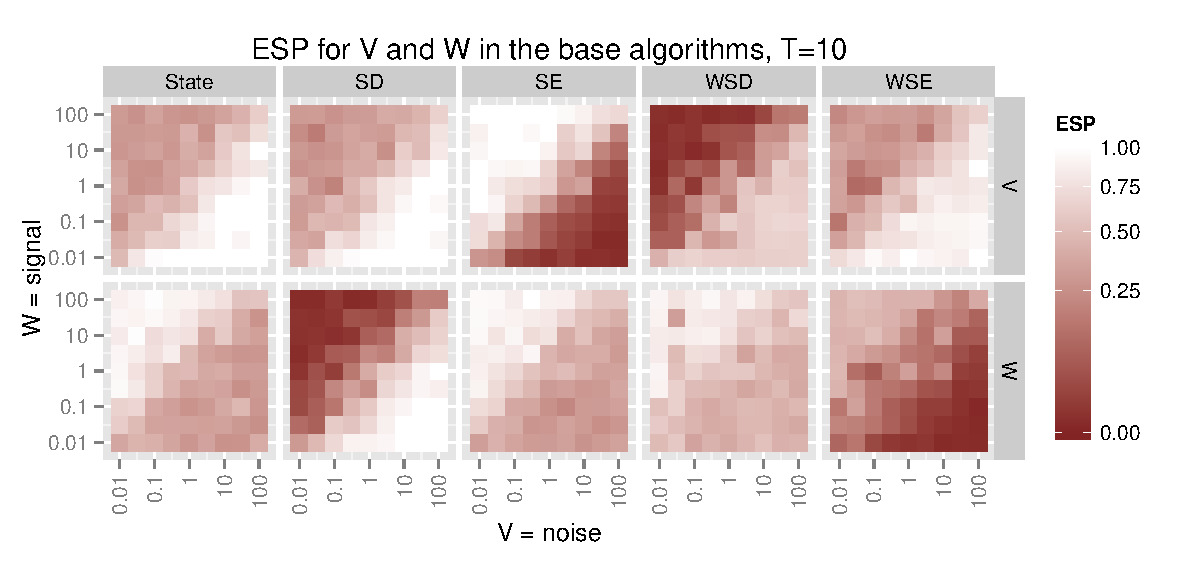
\includegraphics[width=0.48\textwidth]{../plots/baseESplot10}
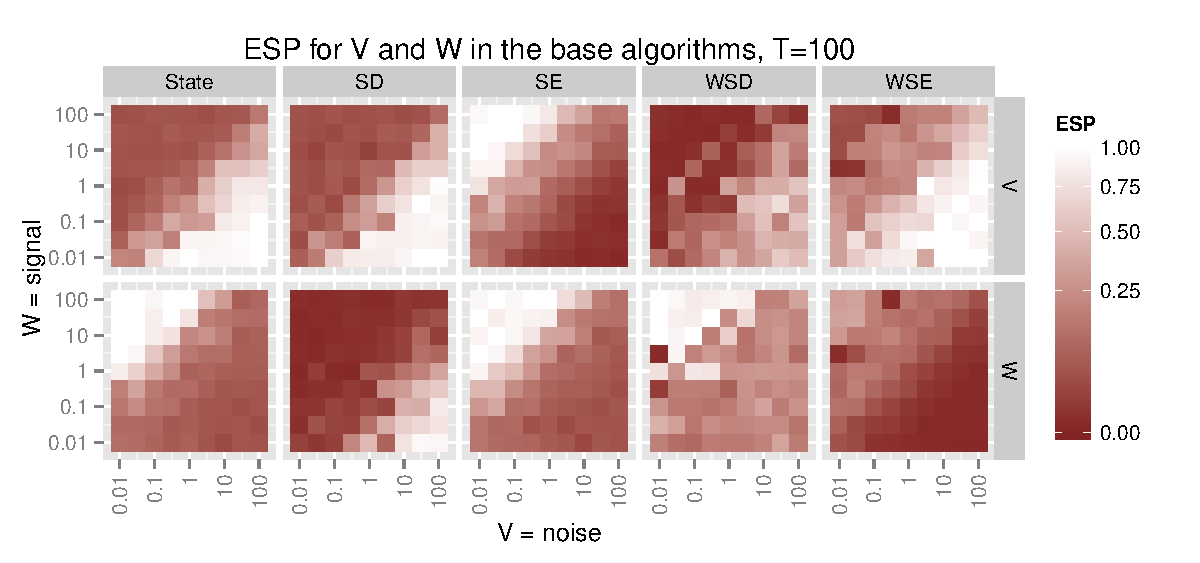
\includegraphics[width=0.48\textwidth]{../plots/baseESplot100}
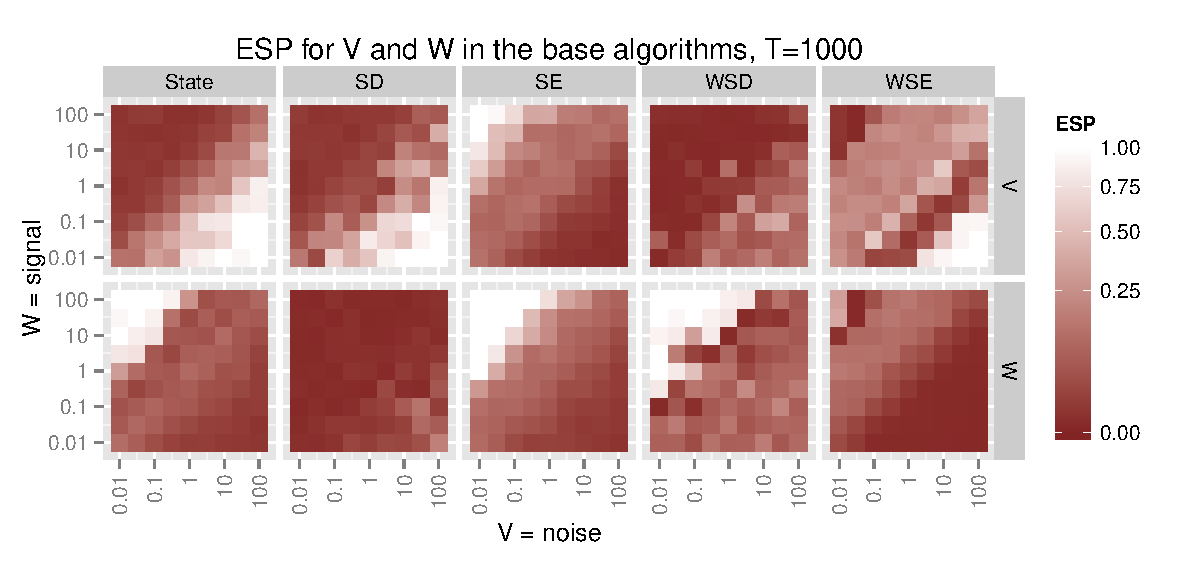
\includegraphics[width=0.48\textwidth]{../plots/baseESplot1000}
\caption{Effective sample proportion in the posterior sampler for a time series of length $T=10$, $T=100$, and $T=1000$, for $V$ and $W$ in the base samplers. $X$ and $Y$ axes indicate the true values of $V$ and $W$ respectively for the simulated data. Note that the signal-to-noise ratio is constant moving up any diagonal. In the upper left the signal is high, in the lower right the noise is high.}
\label{baseESplot}
\end{figure}

\begin{figure}[!ht]
\centering
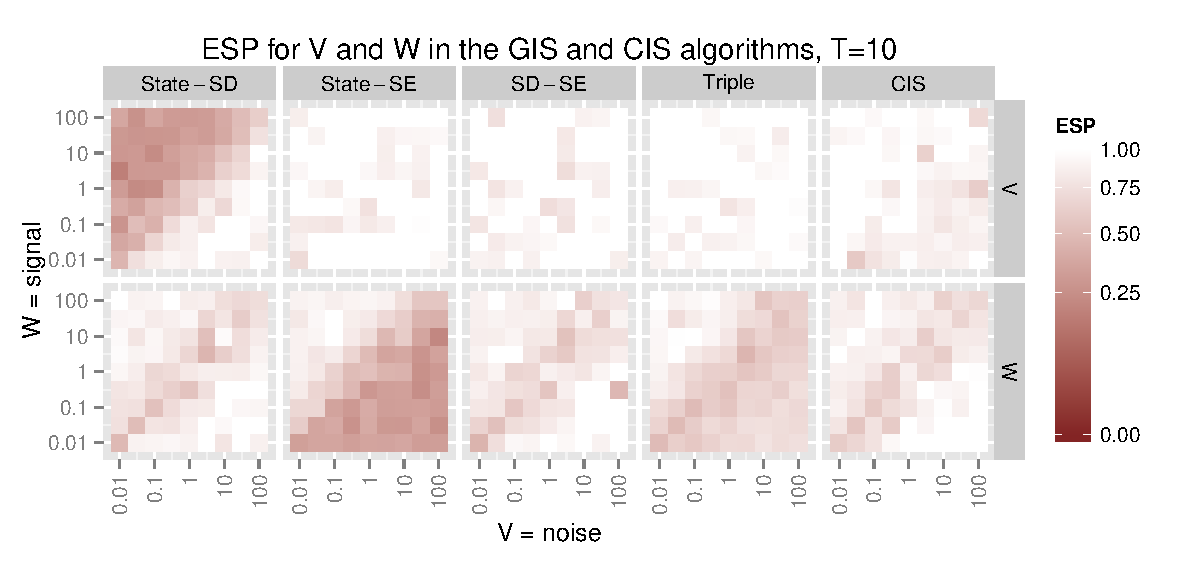
\includegraphics[width=0.48\textwidth]{../plots/intESplot10}
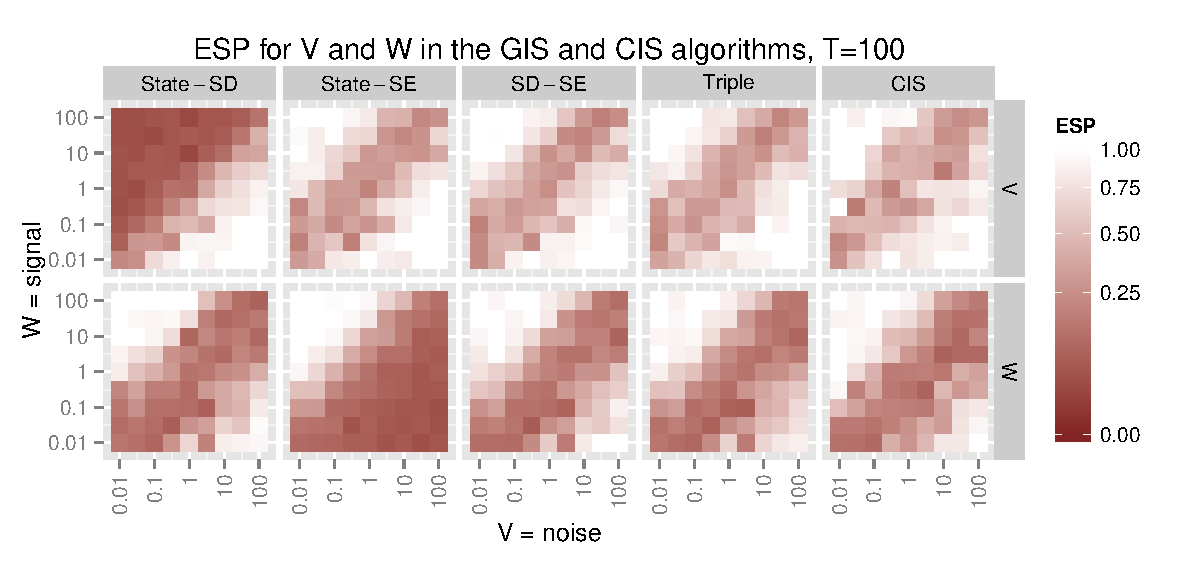
\includegraphics[width=0.48\textwidth]{../plots/intESplot100}
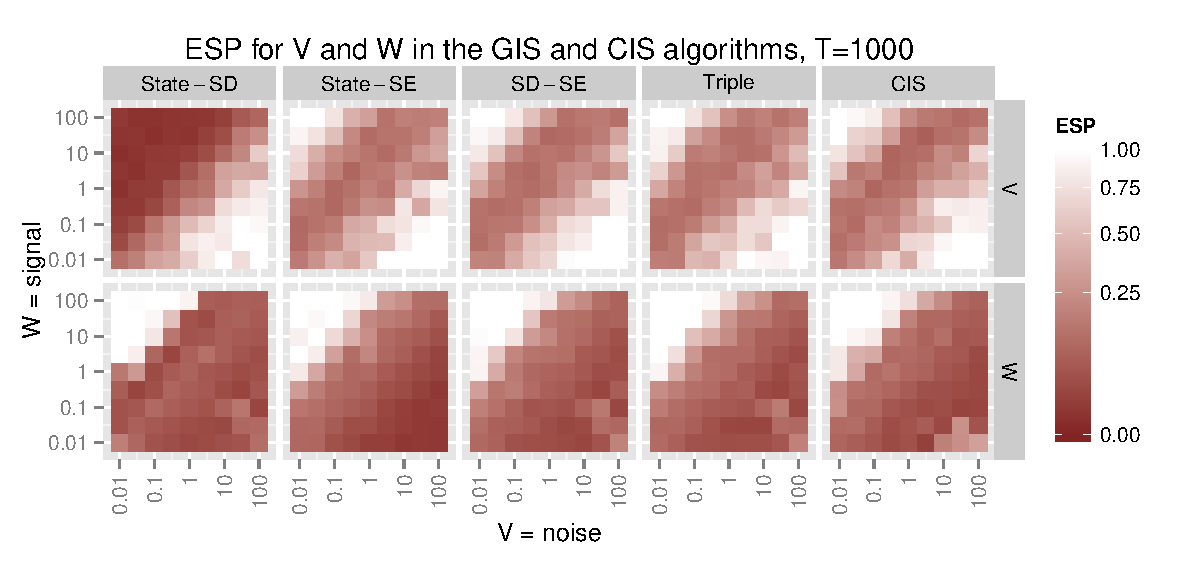
\includegraphics[width=0.48\textwidth]{../plots/intESplot1000}
\caption{ESP in the posterior sampler for $V$ and $W$ in for $T=10$, $T=100$, and $T=1000$ in all four GIS samplers based on any two or three of the states, scaled disturbances and scaled errors as well as the CIS sampler.}
\label{intESplot}
\end{figure}

\begin{figure}[!ht]
\centering
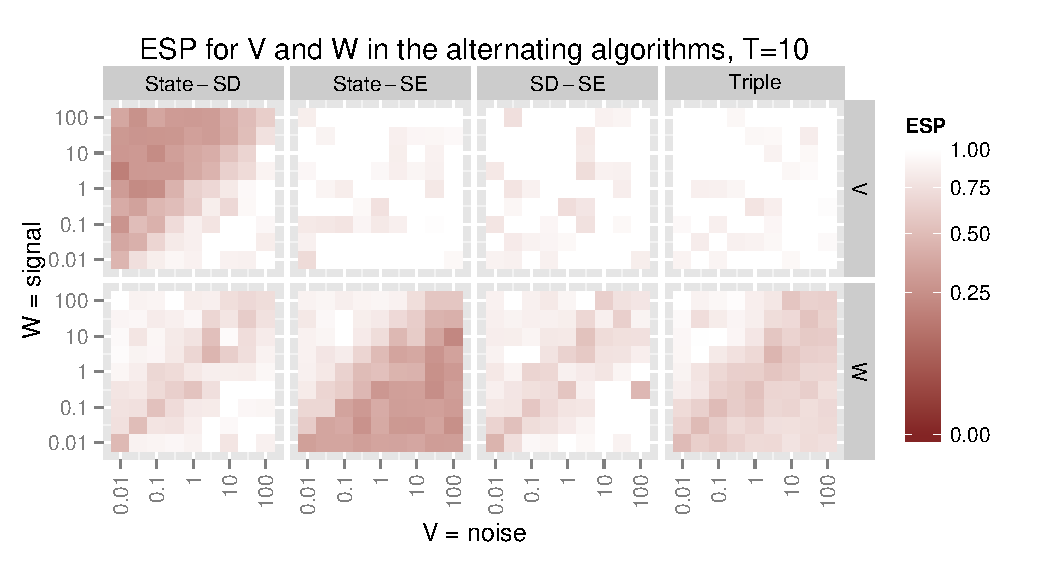
\includegraphics[width=0.48\textwidth]{../plots/altESplot10}
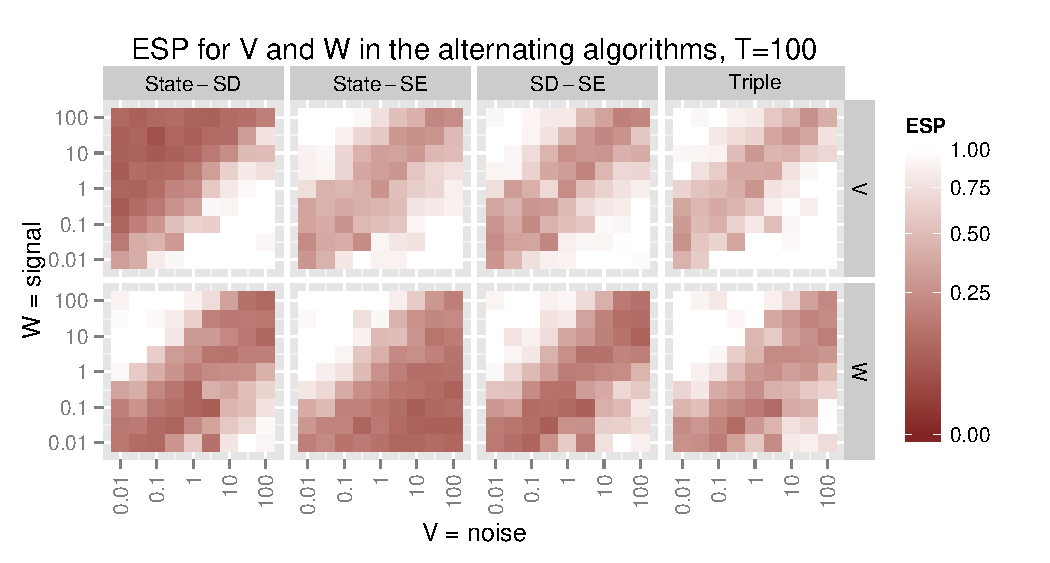
\includegraphics[width=0.48\textwidth]{../plots/altESplot100}
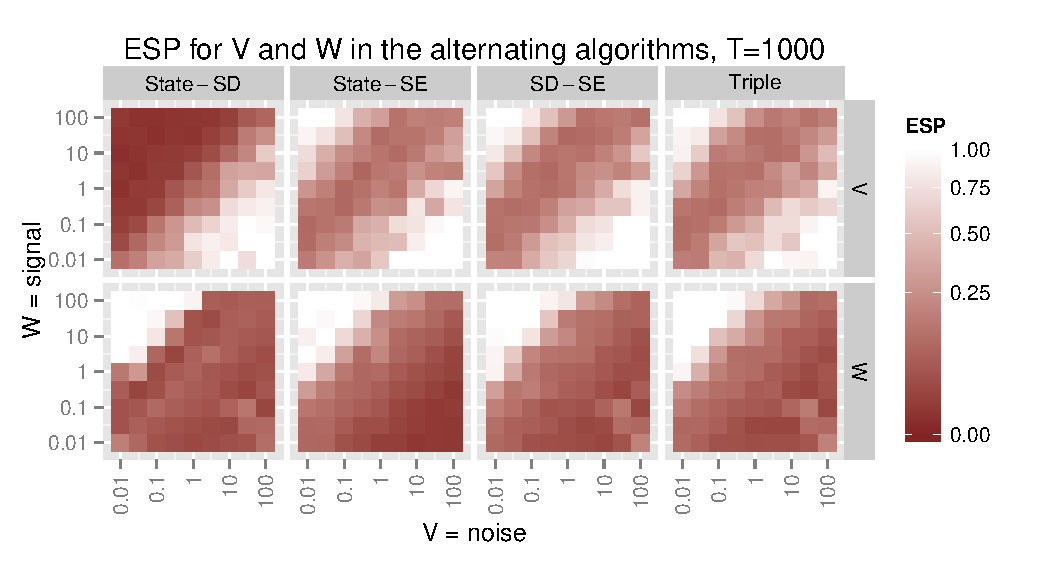
\includegraphics[width=0.48\textwidth]{../plots/altESplot1000}
\caption{ESP in the posterior sampler for $V$ and $W$ for $T=10$, $T=100$, and $T=1000$ in all four alternating samplers based on any two or three of the states, scaled disturbances and scaled errors.}
\label{altESplot}
\end{figure}

\begin{figure}[!ht]
\centering
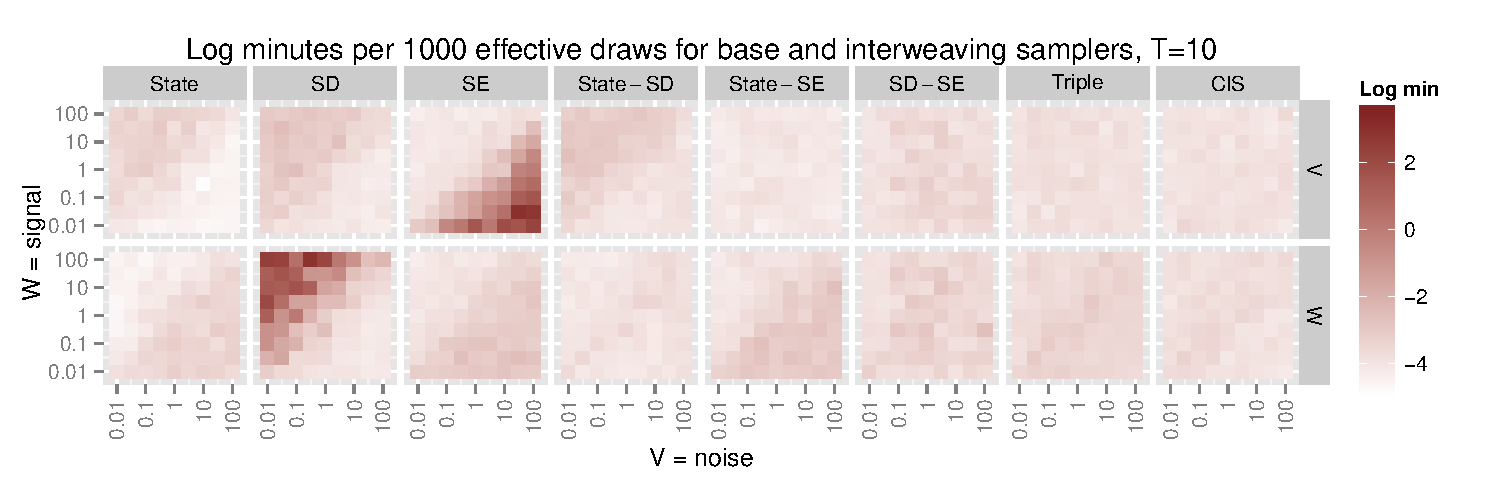
\includegraphics[width=0.8\textwidth]{../plots/baseinttimeplot10}
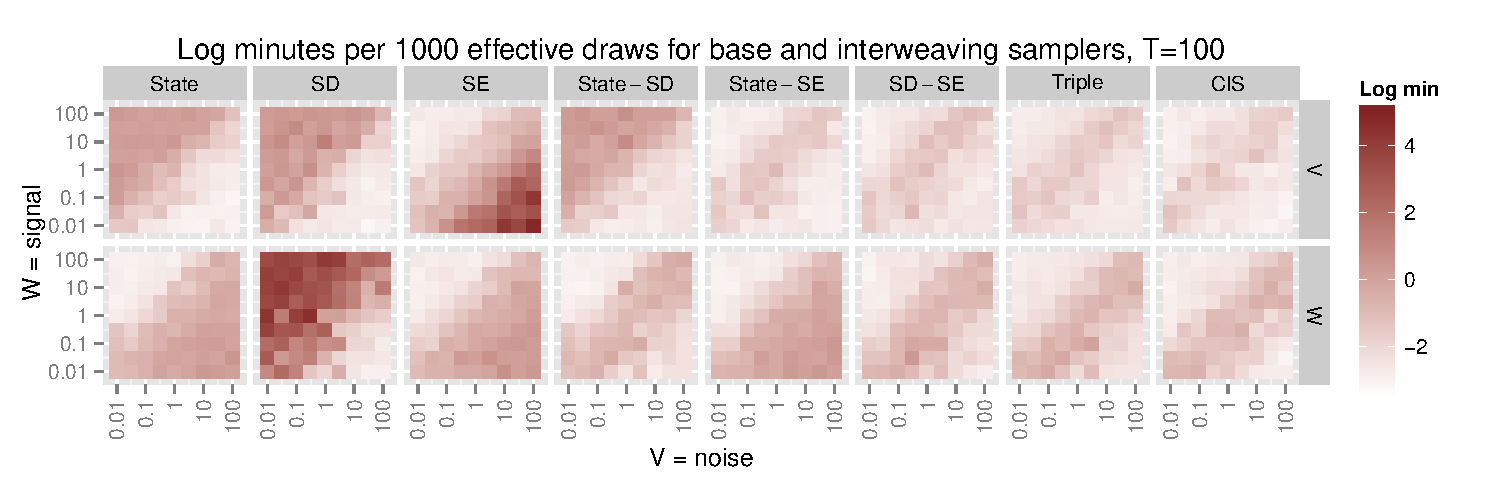
\includegraphics[width=0.8\textwidth]{../plots/baseinttimeplot100}
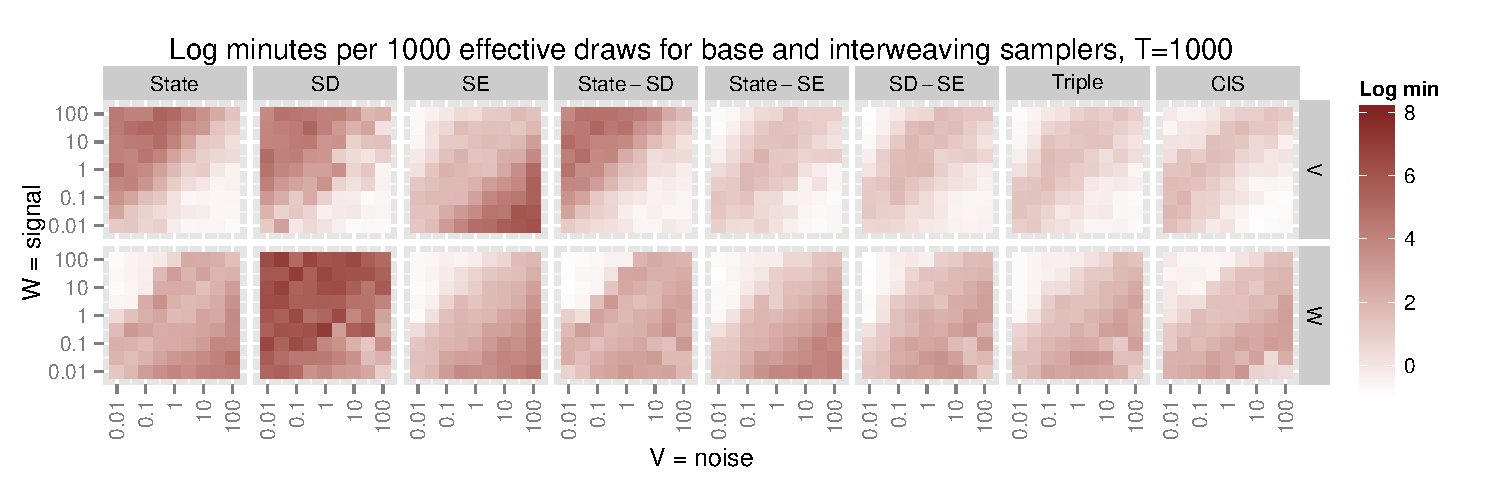
\includegraphics[width=0.8\textwidth]{../plots/baseinttimeplot1000}
\caption{Log of the time in minutes per 1000 effective draws in the posterior sampler for $V$ and $W$, for $T=10$, $T=100$, and $T=1000$ in the state, scaled disturbance and scaled error samplers and for all five interweaving samplers. Note that the scale changes as $T$ changes.}
\label{baseinttimeplot}
\end{figure}


\begin{figure}[!ht]
\centering
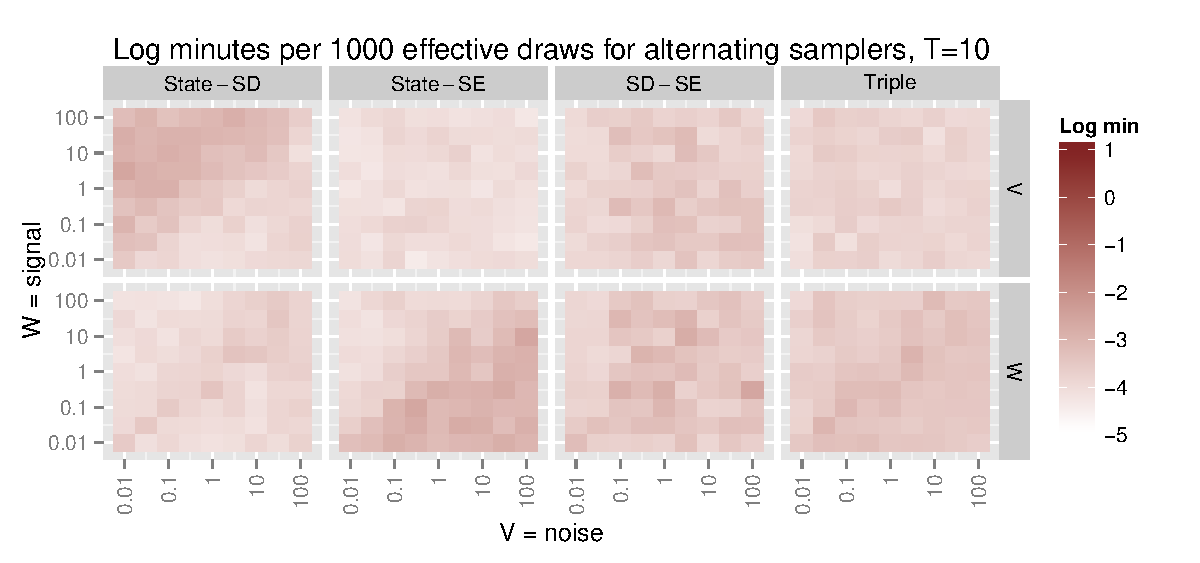
\includegraphics[width=0.48\textwidth]{../plots/altinttimeplot10}
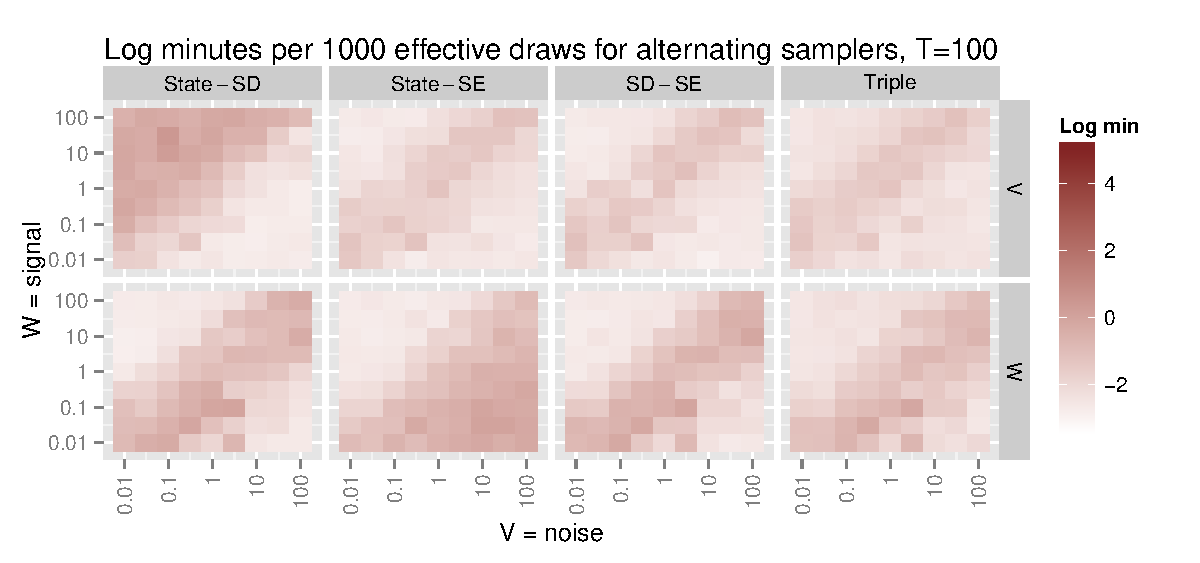
\includegraphics[width=0.48\textwidth]{../plots/altinttimeplot100}
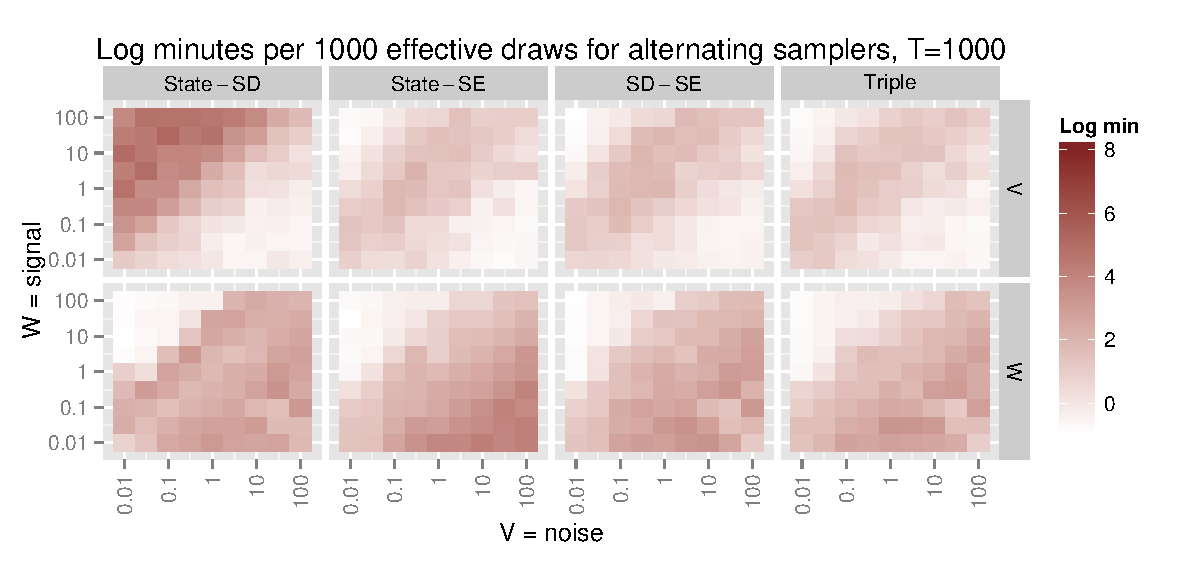
\includegraphics[width=0.48\textwidth]{../plots/altinttimeplot1000}
\caption{Log of the time in minutes per 1000 effective draws in the posterior sampler for $V$ and $W$, for $T=10$, $T=100$, and $T=1000$ in the alternating samplers.}
\label{altinttimeplot}
\end{figure}
\clearpage
\bibliographystyle{ECA_jasa}  % proper bibliography style for ASA
\bibliography{dlmasis}
\end{document}

